\documentclass[main.tex]{subfiles}

\begin{document}

\section{Conclusiones}

Considerando el an\'alisis previamente realizado, se determin\'o que la ecualizaci\'on \'optima del canal se logra con un esquema de inversi\'on de sistema, actualizando los coeficientes del filtro adaptativo mediante el m\'etodo NLMS. Los par\'ametros \'optimos de este procedimiento se determinaron como:

\begin{equation}
\begin{aligned}
	N &= 5 \\
	\mu &= 0.005 \\
	\text{delay} &= 1\, \text{tap}
\end{aligned}
\end{equation}

El m\'etodo recomendado es, pues:

\begin{enumerate}
	\item \textbf{Entrenamiento del canal}: la se\~nal deseada es conocida, y es la entrada
	con 1 tap de delay (para compensar el delay introducido por el sistema) 
	\item \textbf{Transmisi\'on}: 
	\begin{enumerate}
		\item utilizando el \'ultimo valor de $w$, se obtienen 16 valores de $y$
		\item se realiza el test expresado en la ecuaci\'on \ref{eq:bayes}
		\item seg\'un el resultado del test, se obtiene el nuevo valor de $w$, procesando
		nuevamente las \'ultimas 16 muestras, pero esta vez utilizando $d=s_0$ o $d=s_1$
		seg\'un corresponda
	\end{enumerate} 
\end{enumerate}

El bit error rate obtenido en estas condiciones es menor al 5\%, con lo cual para obtener una comunicaci\'on confiable deber\'ia utilizarse una codificaci\'on con detecci\'on y correcci\'on de errores (por ejemplo, Hanning).

A modo ilustrativo, las figuras \ref{fig:out0} a \ref{fig:outf} ilustran los resultados obtenidos en algunas iteraciones de la simulaci\'on.

\begin{figure}[hp]
	\centering
	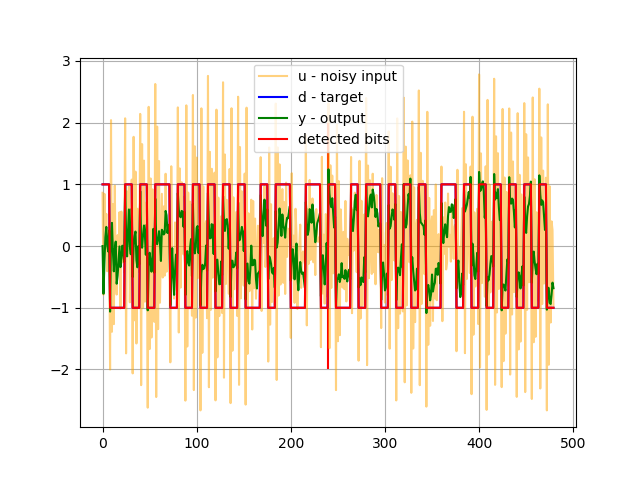
\includegraphics[width=0.5\textwidth]{imagenes/out1.png}
	\caption{Simulaci\'on de la ecualizaci\'on}
	\label{fig:out0}
\end{figure}


\begin{figure}[hp]
	\centering
	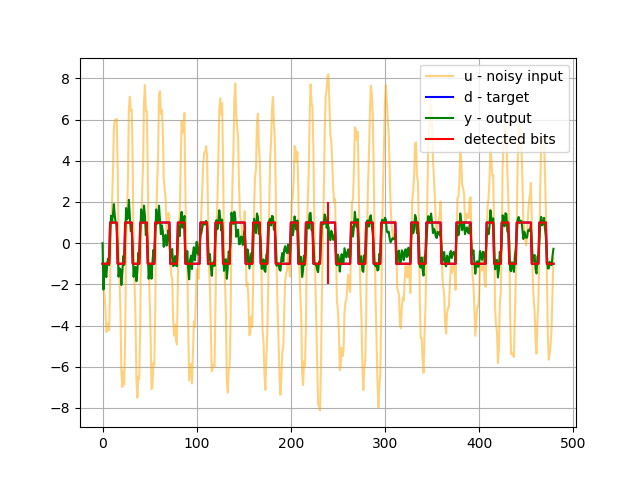
\includegraphics[width=0.5\textwidth]{imagenes/out2.png}
	\caption{Simulaci\'on de la ecualizaci\'on}
\end{figure}


\begin{figure}[hp]
	\centering
	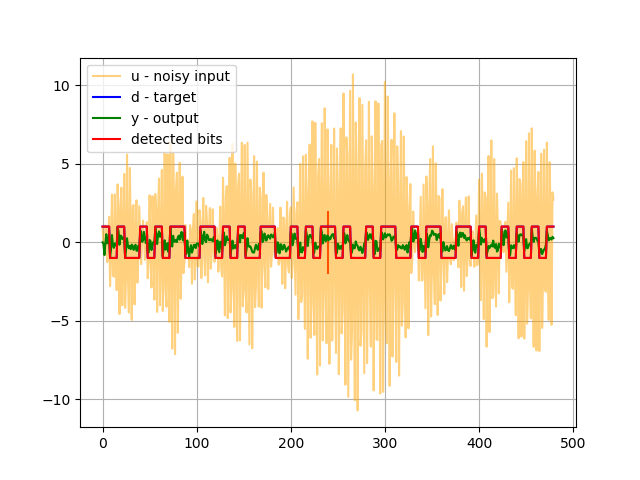
\includegraphics[width=0.5\textwidth]{imagenes/out3.png}
	\caption{Simulaci\'on de la ecualizaci\'on}
\end{figure}


\begin{figure}[hp]
	\centering
	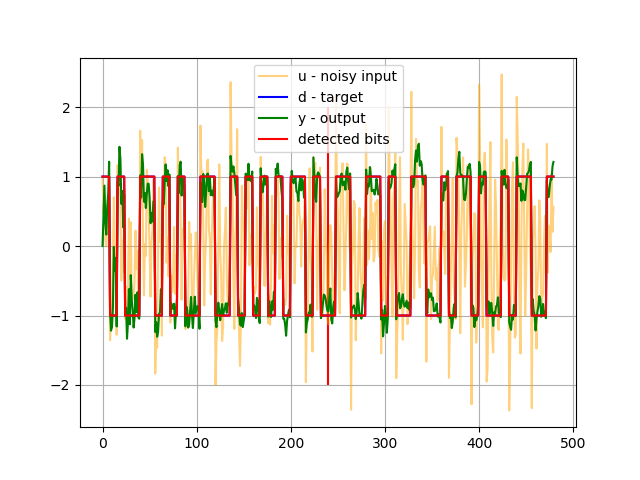
\includegraphics[width=0.5\textwidth]{imagenes/out4.png}
	\caption{Simulaci\'on de la ecualizaci\'on}
\end{figure}


\begin{figure}[hp]
	\centering
	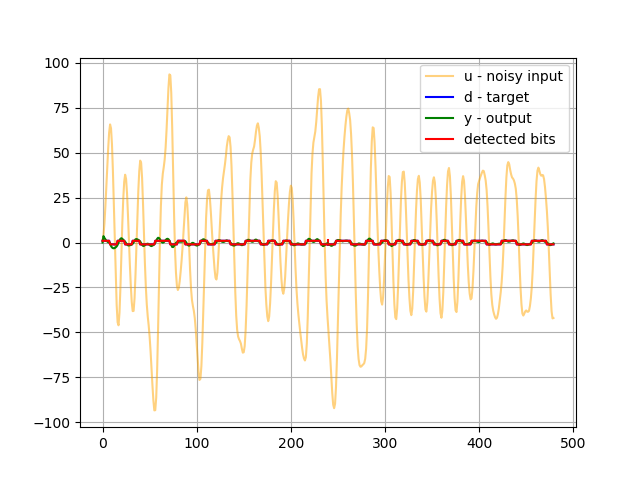
\includegraphics[width=0.5\textwidth]{imagenes/out5.png}
	\caption{5}
\end{figure}

\begin{figure}[hp]
	\centering
	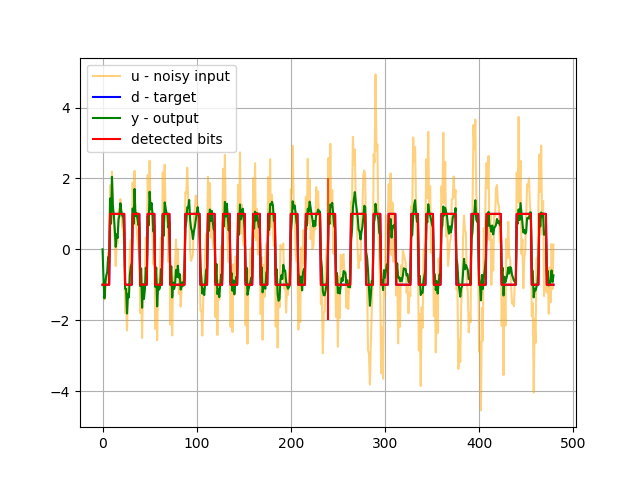
\includegraphics[width=0.5\textwidth]{imagenes/out6.png}
	\caption{Simulaci\'on de la ecualizaci\'on}
\end{figure}



\begin{figure}[hp]
	\centering
	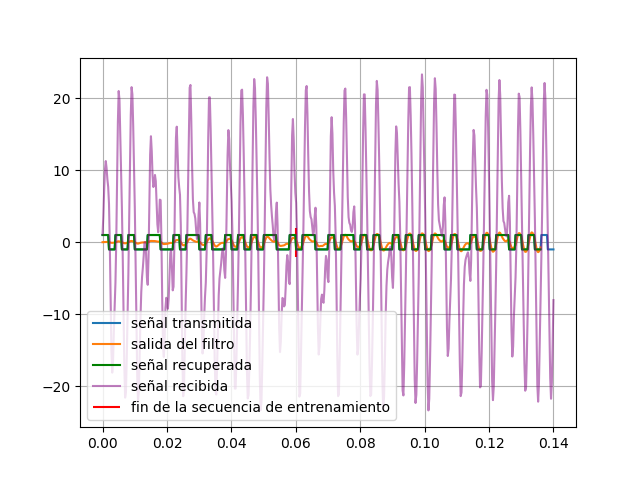
\includegraphics[width=0.5\textwidth]{imagenes/out11.png}
	\caption{Simulaci\'on de la ecualizaci\'on}
\end{figure}


\begin{figure}[hp]
	\centering
	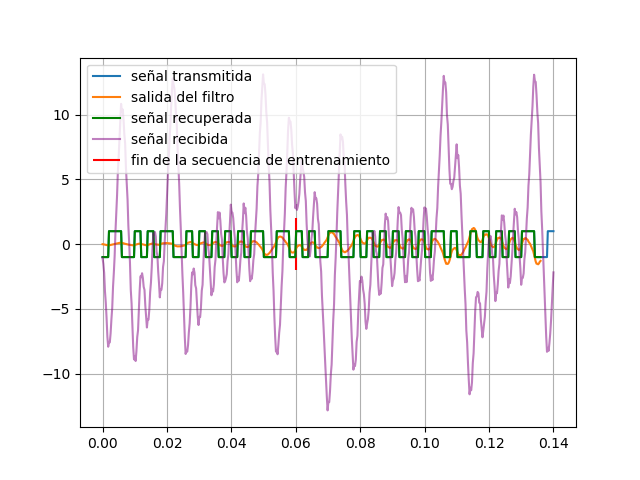
\includegraphics[width=0.5\textwidth]{imagenes/out12.png}
	\caption{Simulaci\'on de la ecualizaci\'on}
\end{figure}

\begin{figure}[hp]
	\centering
	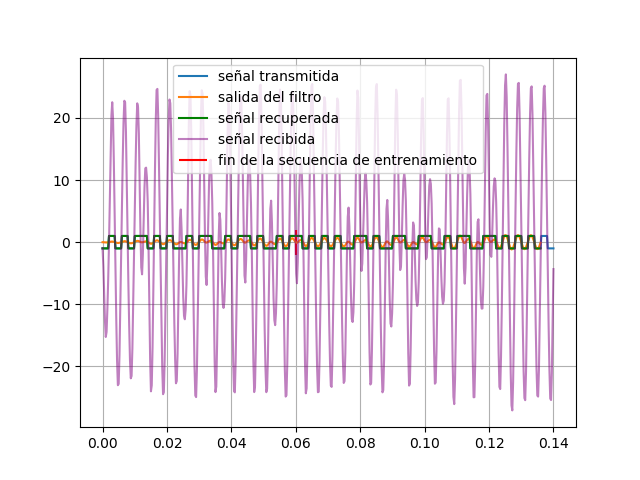
\includegraphics[width=0.5\textwidth]{imagenes/out13.png}
	\caption{Simulaci\'on de la ecualizaci\'on}
	\label{fig:outf}
\end{figure}

\end{document}